\newpage
\section{Serveur multi-agent}
\subsection{Description générale du système}
Le serveur multi-agent a pour but de permettre la dimension collaborative de Colladia.
C'est en effet son rôle d'informer les différents clients éditant un même diagramme des modifications effectuées par les autres utilisateurs.
D'un point de vue technique, le serveur utilise un certain nombre de technologies :
\begin{itemize}
	\item Les requêtes des clients sont reçues via une interface REST implémentée grâce au framework Java Restlet. Cette technologie étant par définition unidirectionnelle, les clients doivent effectuer des requêtes régulières sur le serveur pour être tenus au courant des modifications du diagramme.
	\item Le traitement des requêtes est effectué par un système multi-agent utilisant le framework JADE.
	\item Le contenu des requêtes REST et des messages du SMA sont sérialisés en JSON via la librairie Java Jackson.
\end{itemize}
~\\
La structure du SMA est divisée en deux conteneurs :
\begin{itemize}
	\item Le conteneur principal où résident notamment les agents standards JADE (DF, AMS, etc.) ainsi que l'agent lié au serveur Restlet qui va transformer les requêtes REST reçues en messages pour le SMA (RestAgt). On y trouve aussi l'agent chargé de sauvegarder régulièrement l'état des différents diagrammes dans des fichiers de manière à pouvoir restaurer leur état après un éventuel redémarrage du serveur (SaveAgt).
	\item Le conteneur de diagramme contenant pour chaque diagramme :
	\begin{itemize}
		\item Un ou plusieurs agents élément représentant le diagramme en soi ou des éléments présents dans ce dernier (EltAgt). Ces agents forment entre eux une arborescence dont l'élément représentant le diagramme est la racine.
		\item Un agent horloge responsable de gérer une horloge logique pour la sauvegarde des modifications effectuées sur le diagramme (ClockAgt). L'horloge est initialisée à 0 au démarrage du serveur et est incrémentée de 1 à chaque modification du diagramme ou de ses sous-éléments.
		\item Un agent historique sauvegardant une liste des dernières modifications (HistAgt).
	\end{itemize}
\end{itemize}

\vspace*{\fill}
\begin{figure}[!h]
	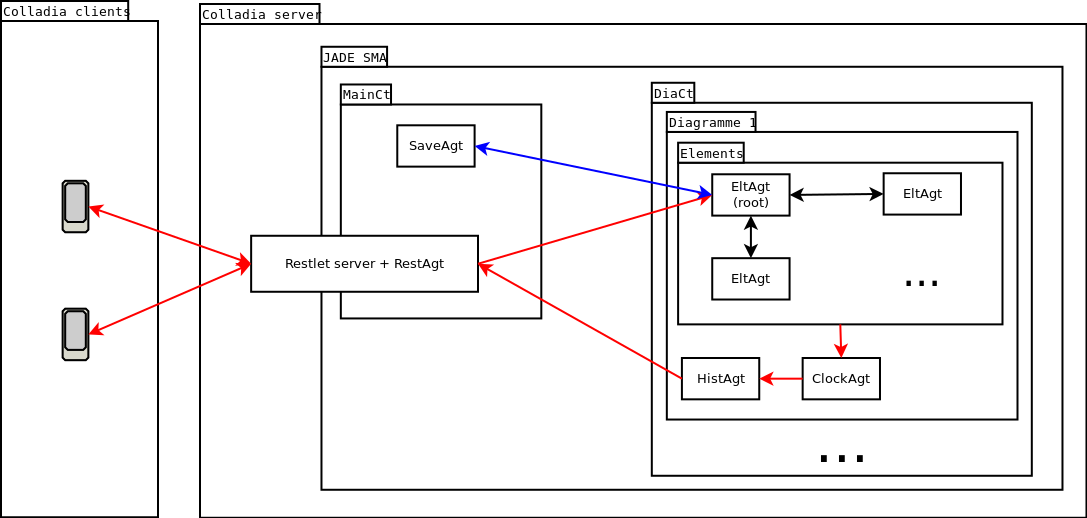
\includegraphics[width=.9\textwidth]{img/general_server}
	\caption{Schéma de l'architecture générale du serveur}
\end{figure}

\subsection{Description de l'interface REST}
\subsubsection{Champs communs}
Un certain nombre de champs sont communs aux différentes requêtes REST.
Pour les entrées le champ \lstinline$last-clock$, optionnel, permettant au serveur de connaître la dernière valeur de l'horloge logique reçue par le client effectuant la requête.

Pour les sorties, il faut commencer par différencier les modifications sauvegardées par l'agent historique du message de retour des requêtes REST.
Le retour comporte obligatoirement un champ \lstinline$status$ contenant un code d'erreur et un champ \lstinline$clock$ donnant la dernière valeur de l'horloge logique du diagramme.
Le champ \lstinline$status$ peut prendre une des valeurs suivantes, inspirées des standards web :
\begin{itemize}
	\item succès (2xx) :
	\begin{itemize}
		\item 200 : OK
	\end{itemize}
	\item redirection (3xx) :
	\begin{itemize}
		\item 304 : non-modifié
	\end{itemize}
	\item erreur client (4xx) :
	\begin{itemize}
		\item 400 : requête mal formée
		\item 401 : existe déjà
		\item 404 : non-trouvé
	\end{itemize}
	\item erreur serveur (5xx) :
	\begin{itemize}
		\item 500 : erreur interne
	\end{itemize}
\end{itemize}
Dans le cas où la requête n'a pas pu être exécutée (\lstinline$status != 200$), un champ \lstinline$error$ est intégré au retour contenant une description de l'erreur.
Si la requête à été exécutée correctement, qu'un champ \lstinline$last-clock$ a été spécifiée par le client et que sa valeur est valide par rapport aux modifications enregistrées par l'HistAgt du diagramme, alors on renvoie un champ \lstinline$modification-list$ qui est un tableau JSON contenant un ensemble de modifications telles que décrites ci-après.
Si on est dans l'incapacité de produire une liste de modifications, on retourne un champ \lstinline$description$ contenant une description complète du diagramme et de ses sous-éléments sous-forme d'une sérialisation JSON.

Les modifications engendrées par certains types de requêtes (PUT, POST et DELETE) et stockées dans l'agent d'historique comportent forcément un champ \lstinline$clock$ indiquant l'horloge à laquelle la modification a eu lieu et un champ \lstinline$type$ donnant le type de la modification (PUT, POST ou DELETE).

\subsubsection{Requêtes GET}
Les requêtes de type GET permettent d'obtenir des informations sur l'état actuel du diagramme et n'engendrent jamais de modifications.
Si l'URI est de la forme \lstinline$<server adress>$, renvoie un champ \lstinline$list$ contenant un tableau JSON des noms des différents diagrammes stockés sur le serveur.

Si l'URI est de la forme \lstinline$<server adress>/<diagram>[/<element> ...]$, renvoie un champ \lstinline$path$ donnant le chemin vers l'élément ciblé sous forme d'un tableau JSON ainsi qu'un champ \lstinline$description$ contenant la description récursive de cet élément.

\subsubsection{Requêtes PUT}
Les requêtes de type PUT permettent de créer de nouveaux diagrammes ou de nouveaux sous-éléments.
Si l'URI est de la forme \lstinline$<server adress>/<diagram>$ c'est une création de diagramme, et dans le cas d'un succès (un diagramme possédant le même nom n'existe pas encore), on renvoie un champ \lstinline$path$ contenant le nom du diagramme.

Si l'URI cible un élément (\lstinline$<server adress>/<diagram>/<element[/<element> ...]>$), on créé un nouveau sous-élément.
La requête peut optionnellement contenir un champ \lstinline$properties$ contenant des couples (propriété, valeur) pour initialiser les propriétés de l’élément.
Le retour contient un champ \lstinline$path$ ainsi qu'un champ \lstinline$properties$ contenant une description des propriétés de l'élément venant d'être créé.

\subsubsection{Requêtes DELETE}
Les requêtes de type DELETE permettent de supprimer un EltAgt ou bien une partie de ses propriétés.
Dans les deux cas, l'URI est de la forme \lstinline$<adrr>/<diagram>[/<element> ...]$.
Si la requête possède un champ \lstinline$properties-list$ contenant une liste de nom de propriété à supprimer, alors on supprime uniquement ces propriétés au niveau de l'élément ciblé.
Sinon, on supprime l'EltAgt ciblé ainsi que tous ses fils récursivement.
Dans les deux cas, la modification a la même forme que la requête initiale, à ceci-près que le chemin de l'URI est intégré dans un champ \lstinline$path$ et le type de la requête dans un champ \lstinline$type$.

\subsubsection{Requêtes POST}
Les requêtes REST de type POST permettent de modifier la valeur des propriétés d'un élément, une option permet d’exécuter un algorithme d'auto-positionnement sur les fils d'un EltAgt ciblé.
Dans les deux cas, l'URI est de la forme \lstinline$<adrr>/<diagram>[/<element> ...]$.
Pour modifier directement des propriétés, un champ \lstinline$properties$ contenant des couples (propriété, valeur) doit être spécifié dans la requête.
La modification possède une forme identique à la requête initiale.

Pour exécuter l'algorithme d'auto-positionnement, il faut spécifier dans la requête un champ \lstinline$options$ associé à une liste JSON contenant une valeur \lstinline$auto-positioning$.
Cette requête induit la sauvegarde de 0+ modifications de type POST, une par fils auto-positionnable. Un fils est dit auto-positionnable si il contient des propriétés suffisantes pour permettre un repositionnement, dans notre cas \lstinline$xMin$, \lstinline$xMax$, \lstinline$yMin$ et \lstinline$yMax$.
Chaque modification enregistrée contient un champ \lstinline$path$ contenant le chemin de l'EltAgt modifié ainsi qu'un champ \lstinline$properties$ récapitulant les altérations effectuées.

\subsection{Description des agents et des comportements}

\subsection{Description générale des messages}

% \subsection{Description détaillée des fonctionnalités}
